\documentclass[tikz]{standalone}
\begin{document}
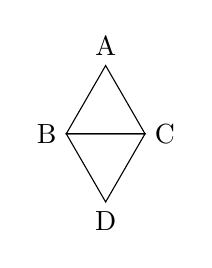
\begin{tikzpicture}
\begin{scope}
\draw (0,0) -- (1,0) -- (0.5,0.866) -- cycle;
\draw (0,0) -- (1,0) -- (0.5,-0.866) -- cycle;
\end{scope}
\begin{scope}
\draw (0.5,0.866) [above] node{A};
\draw (0,0) [left] node{B};
\draw (1,0) [right] node{C};
\draw (0.5,-0.866) [below] node{D};
\end{scope}
\end{tikzpicture}
\end{document}
